\chapter{ETAT DE L'ART}
\begin{spacing}{1.2}
\minitoc
\thispagestyle{MyStyle}
\end{spacing}
\newpage

\section{Introduction}
Ce chapitre présente un aperçu des avancées dans l'analyse sémantique des images et le Web sémantique. En détaillant les concepts de base, les techniques de détection d'objets, de classification, de segmentation sémantique et de reconnaissance de scènes, ainsi que les méthodes d'annotation des données, il établit les fondements théoriques et pratiques de la recherche actuelle. L'objectif est de fournir une compréhension claire des technologies et approches qui permettent de transformer des images en informations interprétables par les machines.

\section{L'analyse sémantique des images}

\subsection{Definition}
\quad L'analyse sémantique des images est un domaine de l'intelligence artificielle qui vise à comprendre le contenu visuel des images en leur attribuant des significations sémantiques. Contrairement à l'analyse basée uniquement sur des caractéristiques visuelles telles que la couleur, la texture ou la forme, l'analyse sémantique cherche à interpréter le contenu des images de manière similaire à la façon dont les humains le font.

\subsection{Le Web sémantique}
\quad Le Web sémantique est une extension du World Wide Web dans laquelle l'information est structurée de manière à être interprétable par les machines, permettant ainsi aux ordinateurs de comprendre le sens des données et des relations entre elles. Conçu pour rendre les contenus du Web plus intelligibles et exploitables par les machines, le Web sémantique repose sur l'utilisation de formats standardisés (comme RDF, OWL et SPARQL) pour représenter les connaissances de manière formelle et expressive. En utilisant ces standards, le Web sémantique vise à faciliter la recherche d'information avancée, l'intégration de données provenant de sources diverses, le raisonnement automatique et le développement d'applications intelligentes. En résumé, le Web sémantique vise à transformer le Web en une vaste base de connaissances interconnectée, où les données sont organisées et structurées de manière à être accessibles, compréhensibles et utilisables par les machines.

\subsection{Rapport entre L'analyse sémantique des images et le Le Web sémantique}
Le rapport entre le Web sémantique et l'analyse sémantique des images réside dans leur objectif commun de donner un sens aux données de manière structurée et interprétable par les machines. \\

\textemdash \textbf{ Représentation des connaissances :}
\begin{itemize}
	\item Le Web sémantique utilise des langages comme RDF et OWL pour représenter les connaissances de manière formelle et structurée.
	\item Dans l'analyse sémantique des images, les données visuelles extraites des images sont représentées de manière sémantique en utilisant des structures telles que des ontologies ou des modèles de données.
\end{itemize}

\textemdash \textbf{ Le Web sémantique :}
\begin{itemize}
	\item Le Web sémantique vise à donner un sens aux données sur le World Wide Web en utilisant des standards et des technologies pour définir des relations sémantiques entre les données.
	\item l permet l'interopérabilité des données et facilite leur partage et leur intégration entre différentes sources.
\end{itemize}

\textemdash \textbf{ L'analyse sémantique des images :}
\begin{itemize}
	\item L'analyse sémantique des images consiste à attribuer des significations sémantiques aux données visuelles, comme les objets, les scènes et les relations entre eux.
	\item Elle utilise les principes du Web sémantique pour interpréter le contenu des images de manière automatique et significative, permettant des applications avancées telles que la recherche d'images sémantique et la génération automatique de descriptions d'images.
\end{itemize}

\section{Annotation de Données}
\subsection{Definition}
\quad L'annotation de données est le processus consistant à ajouter des métadonnées, des balises ou des étiquettes à des données, telles que des images, des vidéos, des textes, etc., afin de les rendre compréhensibles et utilisables par des systèmes informatiques, notamment des modèles d'apprentissage automatique. Ces métadonnées ajoutées fournissent des informations supplémentaires sur les données, telles que la classe d'un objet dans une image, la catégorie d'un texte, la séquence temporelle dans une vidéo, etc.


\begin{figure}[htbp]
	\begin{center}
		\begin{minipage}[b]{0.7\textwidth}
			\centering
			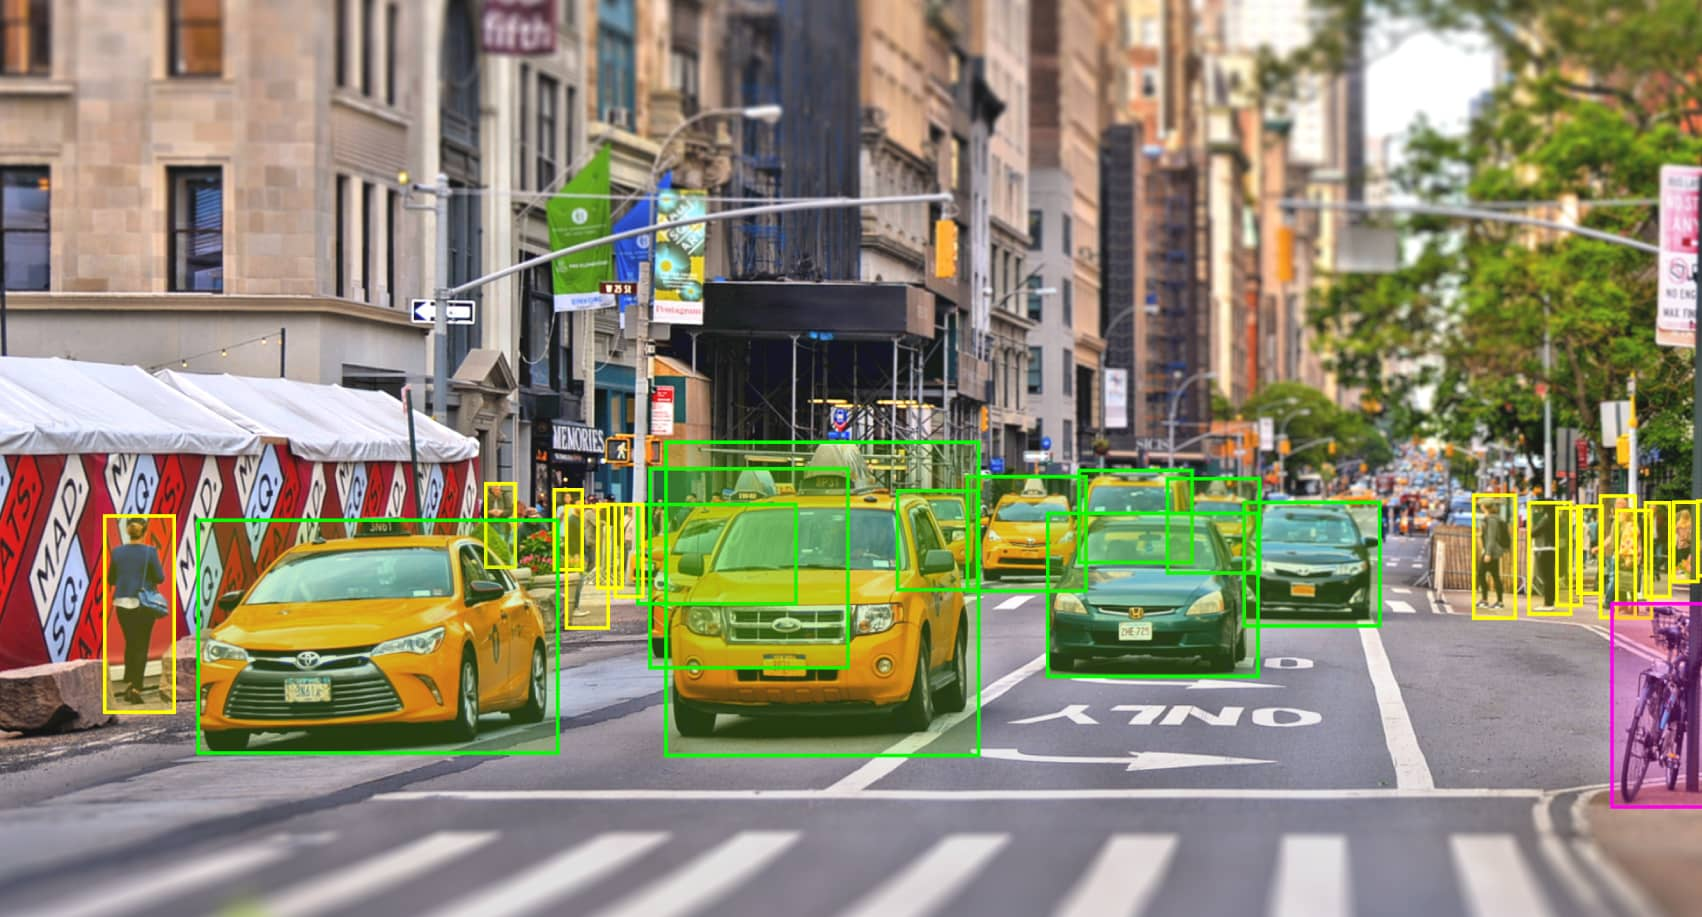
\includegraphics[width=\textwidth]{images/13.jpeg}
			\caption{Illustration d'une annotation de donnée}
		\end{minipage}
	\end{center}
\end{figure}

\subsection{Méthode d'annotation}
\quad Une méthode d'annotation se réfère à l'approche ou à la technique utilisée pour ajouter des informations ou des métadonnées à une image ou à un ensemble de données d'images. Ces informations peuvent inclure des balises, des étiquettes, des régions d'intérêt, des catégories, des contours, des points clés, etc., en fonction de la tâche spécifique à accomplir.

\textemdash \textbf{ Annotation manuelle : }Les annotateurs humains ajoutent manuellement des balises ou dessinent des régions autour des objets d'intérêt dans les images à l'aide d'outils logiciels spécifiques.

\textemdash \textbf{ Annotation par points clés :}Les annotateurs marquent des points clés ou des points caractéristiques sur des objets dans les images, ce qui est souvent utilisé pour la détection et la reconnaissance d'objets.

\textemdash \textbf{ Annotation par segmentation :}Les annotateurs créent des masques ou des contours autour des objets dans les images pour délimiter les régions d'intérêt, ce qui est couramment utilisé pour la segmentation sémantique.

\textemdash \textbf{ Annotation par classification : }Les annotateurs attribuent des étiquettes ou des catégories à des images entières ou à des parties spécifiques des images en fonction de leur contenu ou de leur classe.

\textemdash \textbf{ Annotation par localisation : }Les annotateurs définissent des boîtes englobantes autour des objets d'intérêt pour indiquer leur emplacement et leur taille dans l'image, ce qui est utilisé pour la détection d'objets. \\

Ces méthodes peuvent être utilisées individuellement ou combinées en fonction des besoins de la tâche d'annotation spécifique.

\subsection{Outils d'annotation}
Les outils d'annotation sont des logiciels utilisés pour marquer et étiqueter des éléments spécifiques dans des données comme des images, vidéos ou documents. Ils ajoutent des informations telles que la localisation, les contours et les classes d'objets. L'annotation peut être manuelle ou automatique via des algorithmes d'apprentissage automatique. Les données annotées sont cruciales pour entraîner des modèles d'apprentissage supervisé en fournissant des exemples étiquetés pour l'apprentissage. Voici trois solutions d'annotation automatique :

\begin{itemize}
	\item \textbf{LabelMe :}\\
		\textbf{Forces :}
		\begin{itemize}
			\item \textit{Segmentation sémantique :} Permet des annotations précises pour la segmentation d'images.
			\item \textit{Accessibilité en ligne :} Plateforme en ligne facilitant l'accès et l'utilisation collaborative.
			\item \textit{Diversité des tâches d'annotation :} Prend en charge la détection d'objets et d'autres types d'annotations.
		\end{itemize}
		\textbf{Faiblesses :}
		\begin{itemize}
			\item \textit{Interface utilisateur vieillissante :} L'interface peut sembler obsolète par rapport à des outils plus modernes.
			\item \textit{Limité en fonctionnalités avancées :} Moins de fonctionnalités avancées par rapport à d'autres outils comme Labelbox.
		\end{itemize}
	
	\item \textbf{COCO Annotator :} \\
		\textbf{Forces :}
		\begin{itemize}
			\item \textit{Conçu pour le format COCO :} Spécialement adapté pour les annotations COCO, un format largement utilisé dans la recherche en vision par ordinateur.
			\item \textit{Open-source et personnalisable :} Permet des ajustements et des personnalisations selon les besoins spécifiques des utilisateurs.
			\item \textit{Simplicité d'utilisation :} Interface utilisateur simple et intuitive.
		\end{itemize}
		\textbf{Faiblesses :}
		\begin{itemize}
			\item \textit{Fonctionnalités limitées :} Moins de fonctionnalités avancées comparé à des solutions commerciales.
			\item \textit{Documentation et support :} Documentation parfois limitée et moins de support par rapport aux solutions payantes.
		\end{itemize}
	
	\item \textbf{RoboFlow :} \\
		\textbf{Forces :}
		\begin{itemize}
			\item \textit{Flexibilité et personnalisation :} Il offre une interface intuitive et des fonctionnalités personnalisables pour répondre aux besoins variés des utilisateurs.
			\item \textit{Accessibilité et adaptabilité :} RoboFlow est accessible en ligne et compatible avec différents formats de données, permettant une utilisation facile et une intégration dans divers projets.
		\end{itemize}
		\textbf{Faiblesses :}
		\begin{itemize}
			\item \textit{En cours de développement :} Comme il est en cours de développement, RoboFlow peut présenter des bugs ou des fonctionnalités incomplètes lors des premières versions.
			\item \textit{Documentation initiale limitée :} Les ressources d'aide peuvent être moins abondantes au début du déploiement de RoboFlow.
		\end{itemize}
\end{itemize}
\quad Vu ces limites, nous avons décidé de développer un outil répondant spécifiquement à nos besoins, celui d'annoter des images tout en utilisant une ontologie.


\subsection{Gestion d'ontologie}
\subsubsection{Definition}
Une ontologie OWL (Web Ontology Language) est une représentation formelle et structurée de connaissances dans un domaine spécifique, basée sur le Web. Utilisée principalement dans la gestion des connaissances, la sémantique web et l'intelligence artificielle, elle décrit les relations entre les concepts d'un domaine donné. Les ontologies OWL se composent de classes, de propriétés et d'individus, définissant ainsi les ensembles de choses similaires, les relations entre les classes et les instances spécifiques de classes. Elles permettent de formaliser les connaissances de manière interprétable par les machines, facilitant ainsi la recherche, la récupération et l'analyse des informations dans divers domaines tels que la bioinformatique, l'ingénierie des connaissances et la gestion des ressources.
\subsection{Rapport entre une ontologie et le web sémantique}
\begin{itemize}
	\item \textbf{Représentation des connaissances :} Les ontologies sont des structures formelles qui définissent des concepts, des relations et des propriétés dans un domaine particulier. Elles permettent de représenter la connaissance d'un domaine de manière précise et structurée. Le Web sémantique fournit un ensemble de standards et de technologies (comme RDF, OWL et SPARQL) pour représenter et échanger ces ontologies sur le Web, permettant ainsi aux machines de comprendre et d'interpréter les données de manière plus intelligente.
	
	\item \textbf{Interopérabilité des données :} En utilisant des ontologies compatibles avec les standards du Web sémantique, il est possible de créer des données interopérables qui peuvent être partagées et intégrées entre différents systèmes et applications. Cela facilite l'échange de données entre les organisations, les domaines de connaissances et les communautés d'utilisateurs.
	
	\item \textbf{Raisonnement automatique :} Les ontologies permettent de définir des axiomes, des règles et des restrictions sur les données et les concepts d'un domaine. Le Web sémantique fournit des langages et des outils pour réaliser du raisonnement automatique sur ces ontologies, permettant ainsi de déduire de nouvelles connaissances à partir des informations existantes.
	
\end{itemize}

\subsection{Outils de modélisation ontologique}
Il existe plusieurs outils permettant de créer une ontologie:

\begin{itemize}
	\item \textbf{RDFLib:} Une bibliothèque Python pour travailler avec des données RDF, offrant des fonctionnalités pour la création, la manipulation et le stockage de graphes RDF dans des applications Python.
	
	\textbf{Forces :}
	\begin{itemize}
		\item \textit{Facilité d'utilisation :} Interface simple pour travailler avec des données RDF en Python.
		\item \textit{Flexibilité :} Permet la manipulation avancée de graphes RDF dans un environnement de programmation Python.
	\end{itemize}
	
	\textbf{Faiblesses :}
	\begin{itemize}
		\item \textit{Complexité pour les non-programmeurs :} Peut être difficile à utiliser pour ceux qui ne sont pas familiers avec la programmation Python.
	\end{itemize}
	
	\item \textbf{SWRL:} Le langage de règles sémantiques qui permet l'inférence de connaissances à partir de données RDF.
	
	\textbf{Forces :}
	\begin{itemize}
		\item \textit{Inférence de connaissances :} Permet l'inférence de nouvelles connaissances à partir de données RDF existantes.
		\item \textit{Expressivité :} Permet la spécification de règles complexes pour l'analyse sémantique des données RDF.
	\end{itemize}
	
	\textbf{Faiblesses :}
	\begin{itemize}
		\item \textit{Complexité :} L'écriture de règles SWRL peut être complexe et nécessiter une connaissance approfondie des langages de programmation logique.
	\end{itemize}
	
	\item \textbf{Protege:} Un outil de modélisation des ontologies avec une interface utilisateur conviviale, offrant une gamme étendue de fonctionnalités pour la création et la visualisation des ontologies. Il bénéficie également d'une forte communauté de support.
	
	\textbf{Forces :}
	\begin{itemize}
		\item \textit{Interface conviviale :} Interface graphique intuitive pour créer et visualiser des ontologies.
		\item \textit{Large gamme de fonctionnalités :} Offre une variété de fonctionnalités pour la modélisation des ontologies, y compris des plugins pour des besoins spécifiques.
		\item \textit{Communauté de support active :} Bénéficie d'une forte communauté d'utilisateurs et de développeurs pour le support et l'amélioration continue.
	\end{itemize}
	
	\textbf{Faiblesses :}
	\begin{itemize}
		\item \textit{Performance :} Peut être lent avec de grandes ontologies ou des volumes importants de données.
		\item \textit{Complexité pour les nouveaux utilisateurs :} L'apprentissage de toutes les fonctionnalités peut être intimidant pour les nouveaux utilisateurs.
	\end{itemize}
\end{itemize}

Nous avons choisi Protege en raison de sa convivialité, de ses fonctionnalités étendues et de sa communauté de support. Son adaptation spécifique à nos besoins en matière d'annotation d'images basée sur une ontologie en fait l'outil privilégié pour notre projet.


\section{CONCLUSION}
En résumé, l'état de l'art en analyse sémantique des images et Web sémantique montre des avancées significatives dans la compréhension et l'interprétation des contenus visuels. Les progrès dans les techniques d'annotation et les outils de modélisation facilitent la structuration des connaissances. La convergence de ces domaines ouvre la voie à des applications intelligentes, soulignant l'importance de ces technologies pour l'avenir.